\section{Formal Results}
\label{sec:formal-results}

%\begin{itemize}
%	\item Results that we rely on (petri nets, semilinear sets)
%	\item The base algorithm described in math (without any optimizations)
%	\item Time complexity
%	\item proof for correctness of bidirectional pruning
%	\item mathematical description of optimizations
%\end{itemize}




\subsection{The Algorithm (without Optimizations)}

Given a network system \(\mathcal S= (G, L, \mathit{REQ},  \mathit{RESP}, g_0, \delta, \mathit{req}, \mathit{resp})\):  

\begin{enumerate}
	\item  \textbf{Serializability automaton.} 
	We define an NFA 
	\(
	\mathcal A_{\mathrm{ser}}(\mathcal S)=(Q,\Sigma,\delta^A,q_0,F)
	\), with
	\( Q=G,\;F=G,\;q_0=g_0,
	\)
	over an alphabet
	\(
	\Sigma=\{({\color{ForestGreen}\blacklozenge_{\mathit{req}}}/{\color{red}\blacklozenge_{\mathit{resp}}})
	\mid {\color{ForestGreen}\blacklozenge_{\mathit{req}}}\in\mathit{REQ},\;
	{\color{red}\blacklozenge_{\mathit{resp}}}\in\mathit{RESP}\}.
	\)
%	
%	\todo{old}
%	We define an NFA
%	\[
%	\mathcal A_{\mathrm{ser}}(\mathcal S)
%	= \bigl(Q,\Sigma,\delta,q_0,F\bigr),
%	\quad
%	Q = G,\quad F = G \;\;(\text{global states}),\quad
%	q_0 = g_0 \;\;(\text{initial state}),
%	\]
%	\[
%	\Sigma
%	= \Bigl\{
%	({\color{ForestGreen}\blacklozenge_{\mathit{req}}}\,/\,%
%	{\color{red}\blacklozenge_{\mathit{resp}}})
%	\;\Big|\;
%	{\color{ForestGreen}\blacklozenge_{\mathit{req}}}\in\mathit{REQ},\;
%	{\color{red}\blacklozenge_{\mathit{resp}}}\in\mathit{RESP}
%	\Bigr\}.
%	\]
%
We let each transition correspond to a request/response pair:
\(
\delta^A \subseteq Q \times \Sigma \times Q,
\quad q \xrightarrow{{\color{ForestGreen}\blacklozenge_{\mathit{req}}}/{\color{red}\blacklozenge_{\mathit{resp}}}} q'
\),
%old
%\(
%\delta \;\subseteq\; Q \times \Sigma_{	{\color{ForestGreen}\blacklozenge_{\mathit{req}}}\,/\,%
%	{\color{red}\blacklozenge_{\mathit{resp}}}} \times Q,
%\quad
%\bigl(q \xrightarrow{%
%	{\color{ForestGreen}\blacklozenge_{\mathit{req}}}\,/\,%
%	{\color{red}\blacklozenge_{\mathit{resp}}}%
%} q'\bigr),
%\)
%
%\;\Longleftrightarrow\;
%\begin{array}{l}
iff $\mathcal S$ is in global state $q$ and issues a request
$	{\color{ForestGreen}\blacklozenge_{\mathit{req}}}$, then upon some \textit{full serial execution} it eventually transitions to global state  $q'$ and returns response $	{\color{red}\blacklozenge_{\mathit{resp}}}$.
%\end{array}
%\]
%
%
%
%
%
%
%\begin{array}{l}
%	\mathcal S \text{ at global state } q
%	\;\text{issues}\;
%	{\color{ForestGreen}\blacklozenge_{\mathit{req}}},\\[0.5ex]
%	\text{after full completion of the request, it receives}\;
%	{\color{red}\blacklozenge_{\mathit{resp}}},\\[0.5ex]
%	\text{arriving at global state } q'
%\end{array}
%\]
%
%	
	Its language
	\(L(\mathcal A_{\mathrm{ser}}(\mathcal S))\subseteq\Sigma^*\) is exactly the set of serial
	request/response traces.
	Hence, by definition, it holds that applying the Parikh image gives the set of all multisets of request/response pairs obtained by serial executions:
	\(
	\mathsf{Ser}(\mathcal S)
	\;=\;
	\mathsf{Parikh}\bigl(L(\mathcal A_{\mathrm{ser}}(\mathcal S))\bigr)
	\;\subseteq\;\mathbb N^{\Sigma}.
	\)
%	Finally,
%	\(
%	q_0 = g_0
%	\quad\text{(the initial global state of the NS)}
%	\).
	
	
%	\smallskip
\begin{tcolorbox}[colback=black!5!white, colframe=black, boxrule=1pt]
	\textbf{Example.} For Listing~\ref{lst:MotivatingExample2NonSer}, the NS in Fig.~\ref{fig:code2ExampleNS} gives rise to the Serial NFA in Fig.~\ref{fig:code2ExampleNFA}.
	%
	A trace of request/response pairs is accepted by the NFA iff some serial execution of the program induces it.
	%	
Here, serial runs produce only ({\color{ForestGreen}$\blacklozenge_\text{main}$}/{\color{red}$\blacklozenge_1$}), and the only reachable global state is [\texttt{X=0}].
%	Due to the aforementioned construction, a string of request/response pairs is accepted by the NFA iff there exists a serial execution of the NS that induces it.
%
%	As the states encode the global variable values, and the edges encode request/response pairs for all serial executions, the  
%Specifically, in this case --- serial executions can only produce request/response pairs of the type ({\color{ForestGreen}$\blacklozenge_\text{main}$/{\color{red}$\blacklozenge_1$}}). Furthermore, the only global state reachable in serial executions, is [\texttt{X=0}]. 
	%
%	Intuitively, this corresponds to [\texttt{X=0}] being the initial global state, as well as the system's global state after every single packet exits the network in a serial execution.
	\end{tcolorbox}
	%
	\begin{figure}[!htbp]
		\centering
		% 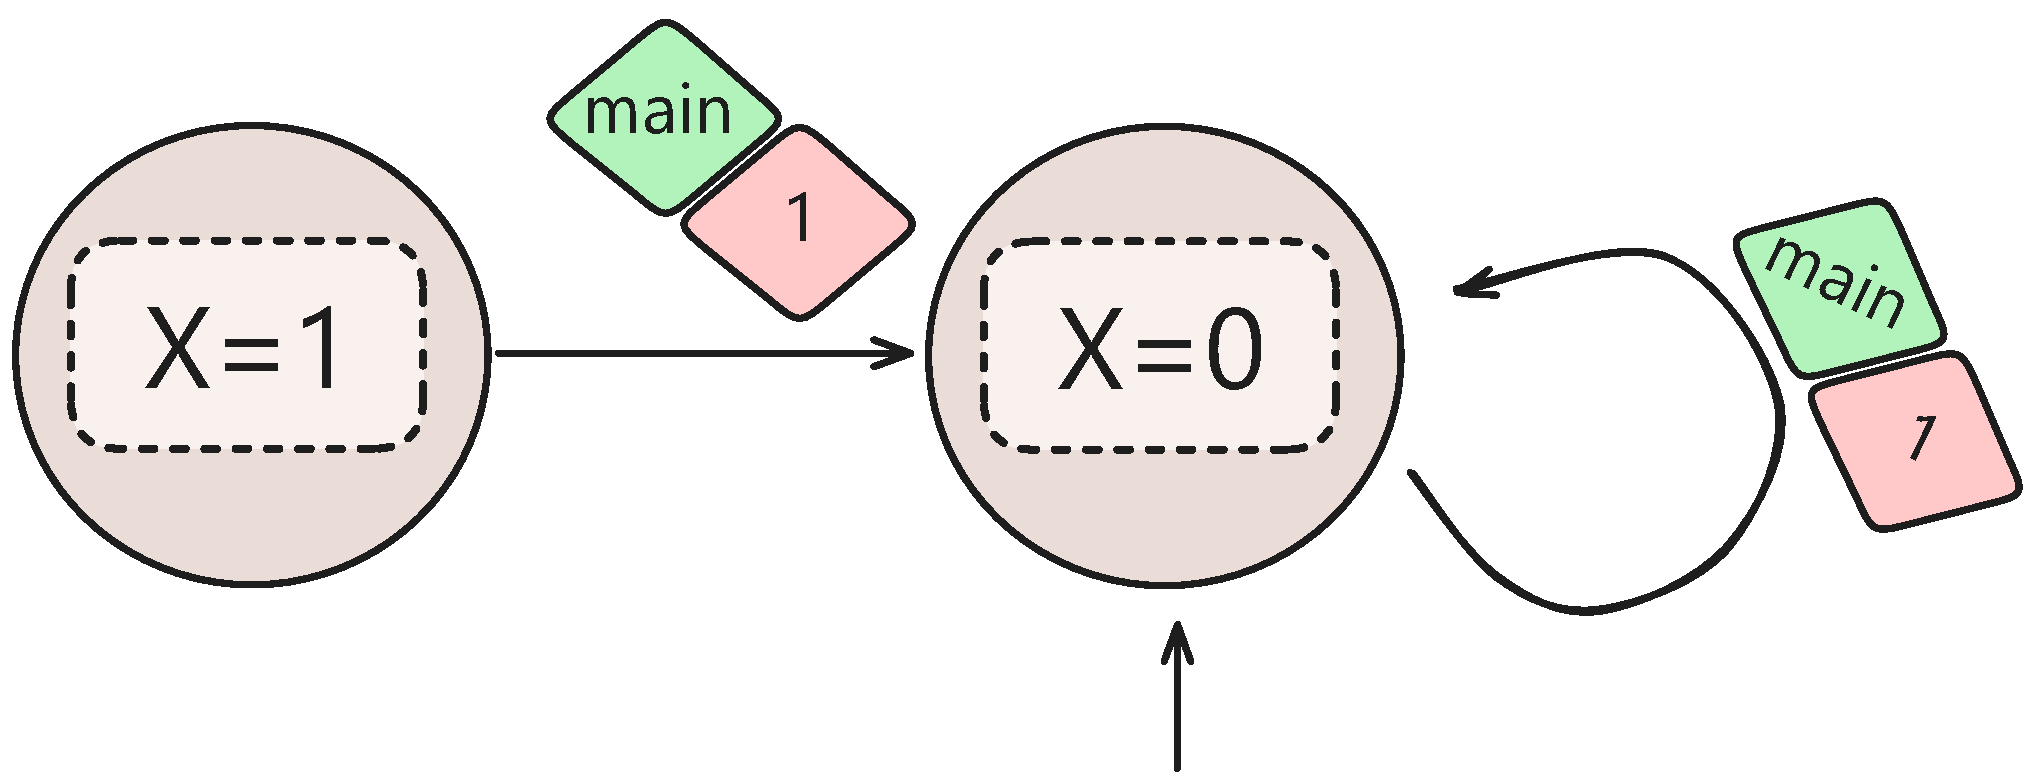
\includegraphics[width=0.48\textwidth,trim=0 0 0 0,clip]{plots/code_2_NFA_v3.pdf}
		
		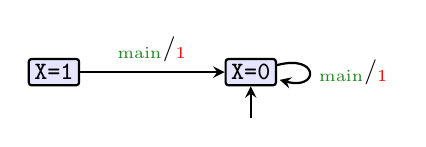
\begin{tikzpicture}[
			->,>=stealth,
			thick,
			node distance=2.5cm,
			state/.style={
				draw=black,
				line width=0.8pt,
				fill=blue!10,
				rectangle,
				rounded corners=1pt,
				inner sep=2pt,
				font=\small
			},
			every node/.style={font=\small}
			]
			% States using the same notation as section 3
			\node[state] (X1) {\texttt{X=1}};
			\node[state, right of=X1] (X0) {\texttt{X=0}};
			
			% Initial state arrow
			\draw[->] ([yshift=-0.4cm]X0.south) -- (X0.south);
			
			% Transitions with proper colored notation from the paper
			\draw[->] (X1) -- node[above] {${\color{ForestGreen}\blacklozenge_{\mathrm{main}}}/{\color{red}\blacklozenge_1}$} (X0);
			\draw[->] (X0) edge[loop right] node[right] {${\color{ForestGreen}\blacklozenge_{\mathrm{main}}}/{\color{red}\blacklozenge_1}$} (X0);
		\end{tikzpicture}
		
		\caption{Serial NFA of Listing~\ref{lst:MotivatingExample2NonSer}.}
		\label{fig:code2ExampleNFA}
	\end{figure}
	
	

	
%	\begin{wrapfigure}{r}{0.50\textwidth}  % “r” = right, width = 0.5\textwidth
%		\centering
%		% 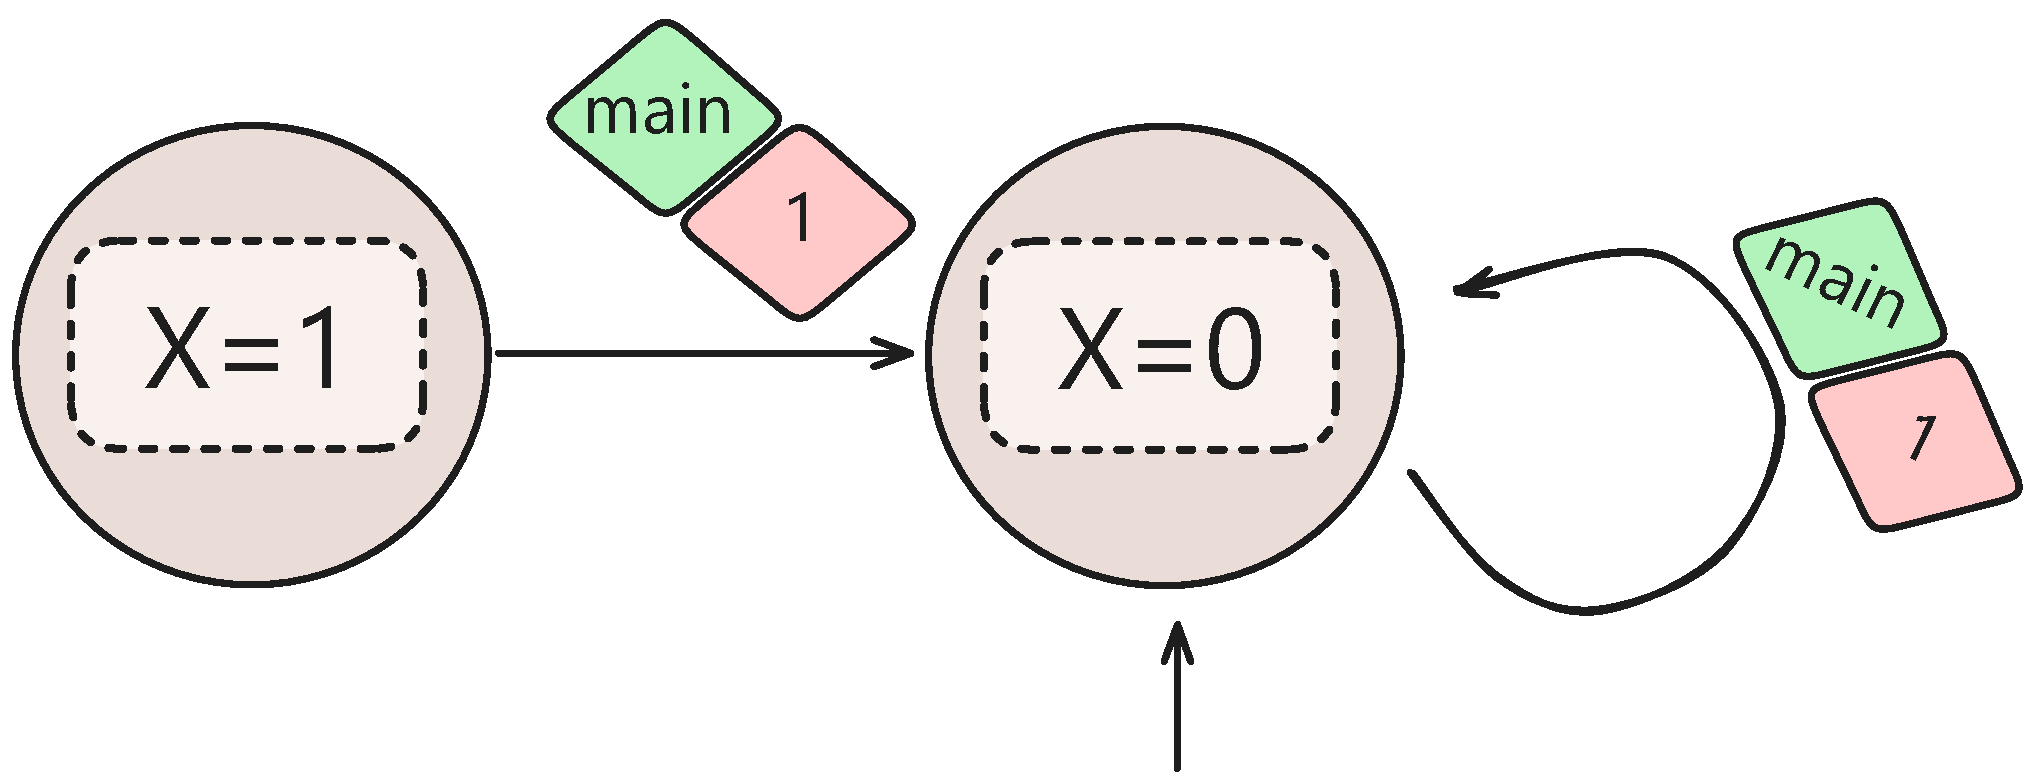
\includegraphics[width=0.48\textwidth,trim=0 0 0 0,clip]{plots/code_2_NFA_v3.pdf}
%		
%		\begin{tikzpicture}[
%			->,>=stealth,
%			thick,
%			node distance=2.5cm,
%			state/.style={
%				draw=black,
%				line width=0.8pt,
%				fill=blue!10,
%				rectangle,
%				rounded corners=1pt,
%				inner sep=2pt,
%				font=\small
%			},
%			every node/.style={font=\small}
%			]
%			% States using the same notation as section 3
%			\node[state] (X1) {\texttt{X=1}};
%			\node[state, right of=X1] (X0) {\texttt{X=0}};
%			
%			% Initial state arrow
%			\draw[->] ([yshift=-0.4cm]X0.south) -- (X0.south);
%			
%			% Transitions with proper colored notation from the paper
%			\draw[->] (X1) -- node[above] {${\color{ForestGreen}\blacklozenge_{\mathrm{main}}}/{\color{red}\blacklozenge_1}$} (X0);
%			\draw[->] (X0) edge[loop right] node[right] {${\color{ForestGreen}\blacklozenge_{\mathrm{main}}}/{\color{red}\blacklozenge_1}$} (X0);
%		\end{tikzpicture}
%		
%		\caption{Serial NFA of Listing~\ref{lst:MotivatingExample2NonSer}.}
%		\label{fig:code2ExampleNFA}
%	\end{wrapfigure}
	%
	%
	%Intuitively, this corresponds to the Listing~\ref{lst:MotivatingExample2NonSer} program updating [X:=1] as an intermediate assignment before yielding.
	
	
	
	\item 
	\textbf{Interleaving Petri net.}
%	
Next, we translate the NS into a Petri net \(N_{\mathrm{int}}(\mathcal S)\). The \textit{non-sink places} of the PN represent either (i) global state assignments, or (ii) local states of in-flight packets. The \textit{sink places} represent request/response pairs of terminating packets.
%
We define the \textit{transitions} between states to correspond to the \(\delta\),\(req\), and \(resp\) mappings of the NS (the \(req\) transitions can fire without any input tokens in order to correspond to initializing arbitrarily many requests externally).
%
Finally, we define the initial marking \(M_0\) to correspond to a single token in the initial global state \(g_0\).
%
This construction (which is fully formalized in Appendix~\ref{appendix:NS-to-PN-formulation}) guarantees that the multiset of all reachable markings \(M\) (with \(M_0 \xrightarrow{}^{*} M\)) projected to the sink places (\(\pi\)), corresponds to the multiset of all  (${{\color{ForestGreen}\blacklozenge_{\mathit{req}}}/{\color{red}\blacklozenge_{\mathit{resp}}}}$) pairs of the NS, as obtained by any interleaving, i.e., \(\mathsf{Int}(\mathcal S)=\{\pi(M) \mid M \in R(N_{\mathrm{int}}(\mathcal S))\}\).



\begin{tcolorbox}[colback=black!5!white, colframe=black, boxrule=1pt]
	\textbf{Example.}
%	\textit{Notation.}
In our running example, the NS gives rise to the PN in Fig.~\ref{fig:code2ExamplePN}, encoding all possible interleavings. The places \textcolor{blue}{ $P_2$} and \textcolor{blue}{$P_3$} represent the global states \textcolor{blue}{[X=1]} and \textcolor{blue}{[X=0]}, respectively, while the places $P_1$, $P_4$, $P_5$, and $P_6$ capture the local states of in-flight requests, i.e., the remaining program code coupled with the assignments to each request’s local variables. Similarly, places \textcolor{red}{$P_7$} and \textcolor{red}{$P_8$} respectively correspond to responses {\color{red}$\blacklozenge_1$} and {\color{red}$\blacklozenge_0$}. Each token either models an active request, a completed request/response pair, or --- when residing in a global-state place --- the current global state of the NS. Finally, transitions implement the network system’s mappings ($\delta/req/resp$): they either spawn a new request (e.g., transition $\textcolor{ForestGreen}{t_1}$, producing {\color{ForestGreen}$\blacklozenge_{\mathrm{main}}$} based on $req$), advance the program by one step (e.g., \(t_2,t_3\), based on $\delta$),
or return a response (e.g., transitions $\textcolor{red}{t_6}$ and $\textcolor{red}{t_7}$, based on $resp$).
\end{tcolorbox}

%Finally, the NS gives rise to the PN in Fig.~\ref{fig:code2ExamplePN}, encoding all possible interleavings.
%%
%The places represent either the global state
%(e.g., places \textcolor{blue}{$P_2$} and \textcolor{blue}{$P_3$} correspond to the global states \textcolor{blue}{[X=1]} and \textcolor{blue}{[X=0]}), while others ($P_1,P_4,P_5,P_6$) correspond to the local state of an in-flight request, i.e., combinations of ``remaining'' programs  assignments to local variables of in-flight requests.
%%
%Furthermore, some requests correspond to responses, e.g., places \textcolor{red}{$P_7$} and \textcolor{red}{$P_8$} corresponds to {\color{red}$\blacklozenge_1$} and {\color{red}$\blacklozenge_0$}.
%%
%Each token corresponds either to a single in-flight request, a single terminated pair of request/response, or (in the case of the global-variable-encoding places), to the current global state.
%%
%Finally, transitions represent the network system's $\delta$ mapping --- encoding either a ``step'' of our program, or spawning a request ($t_1$, which  corresponds to spawning {\color{ForestGreen}$\blacklozenge_\text{main}$}), or returning a response (e.g. transitions $t_6,t_7$).
%


\begin{figure}[!htbp]
	\centering
	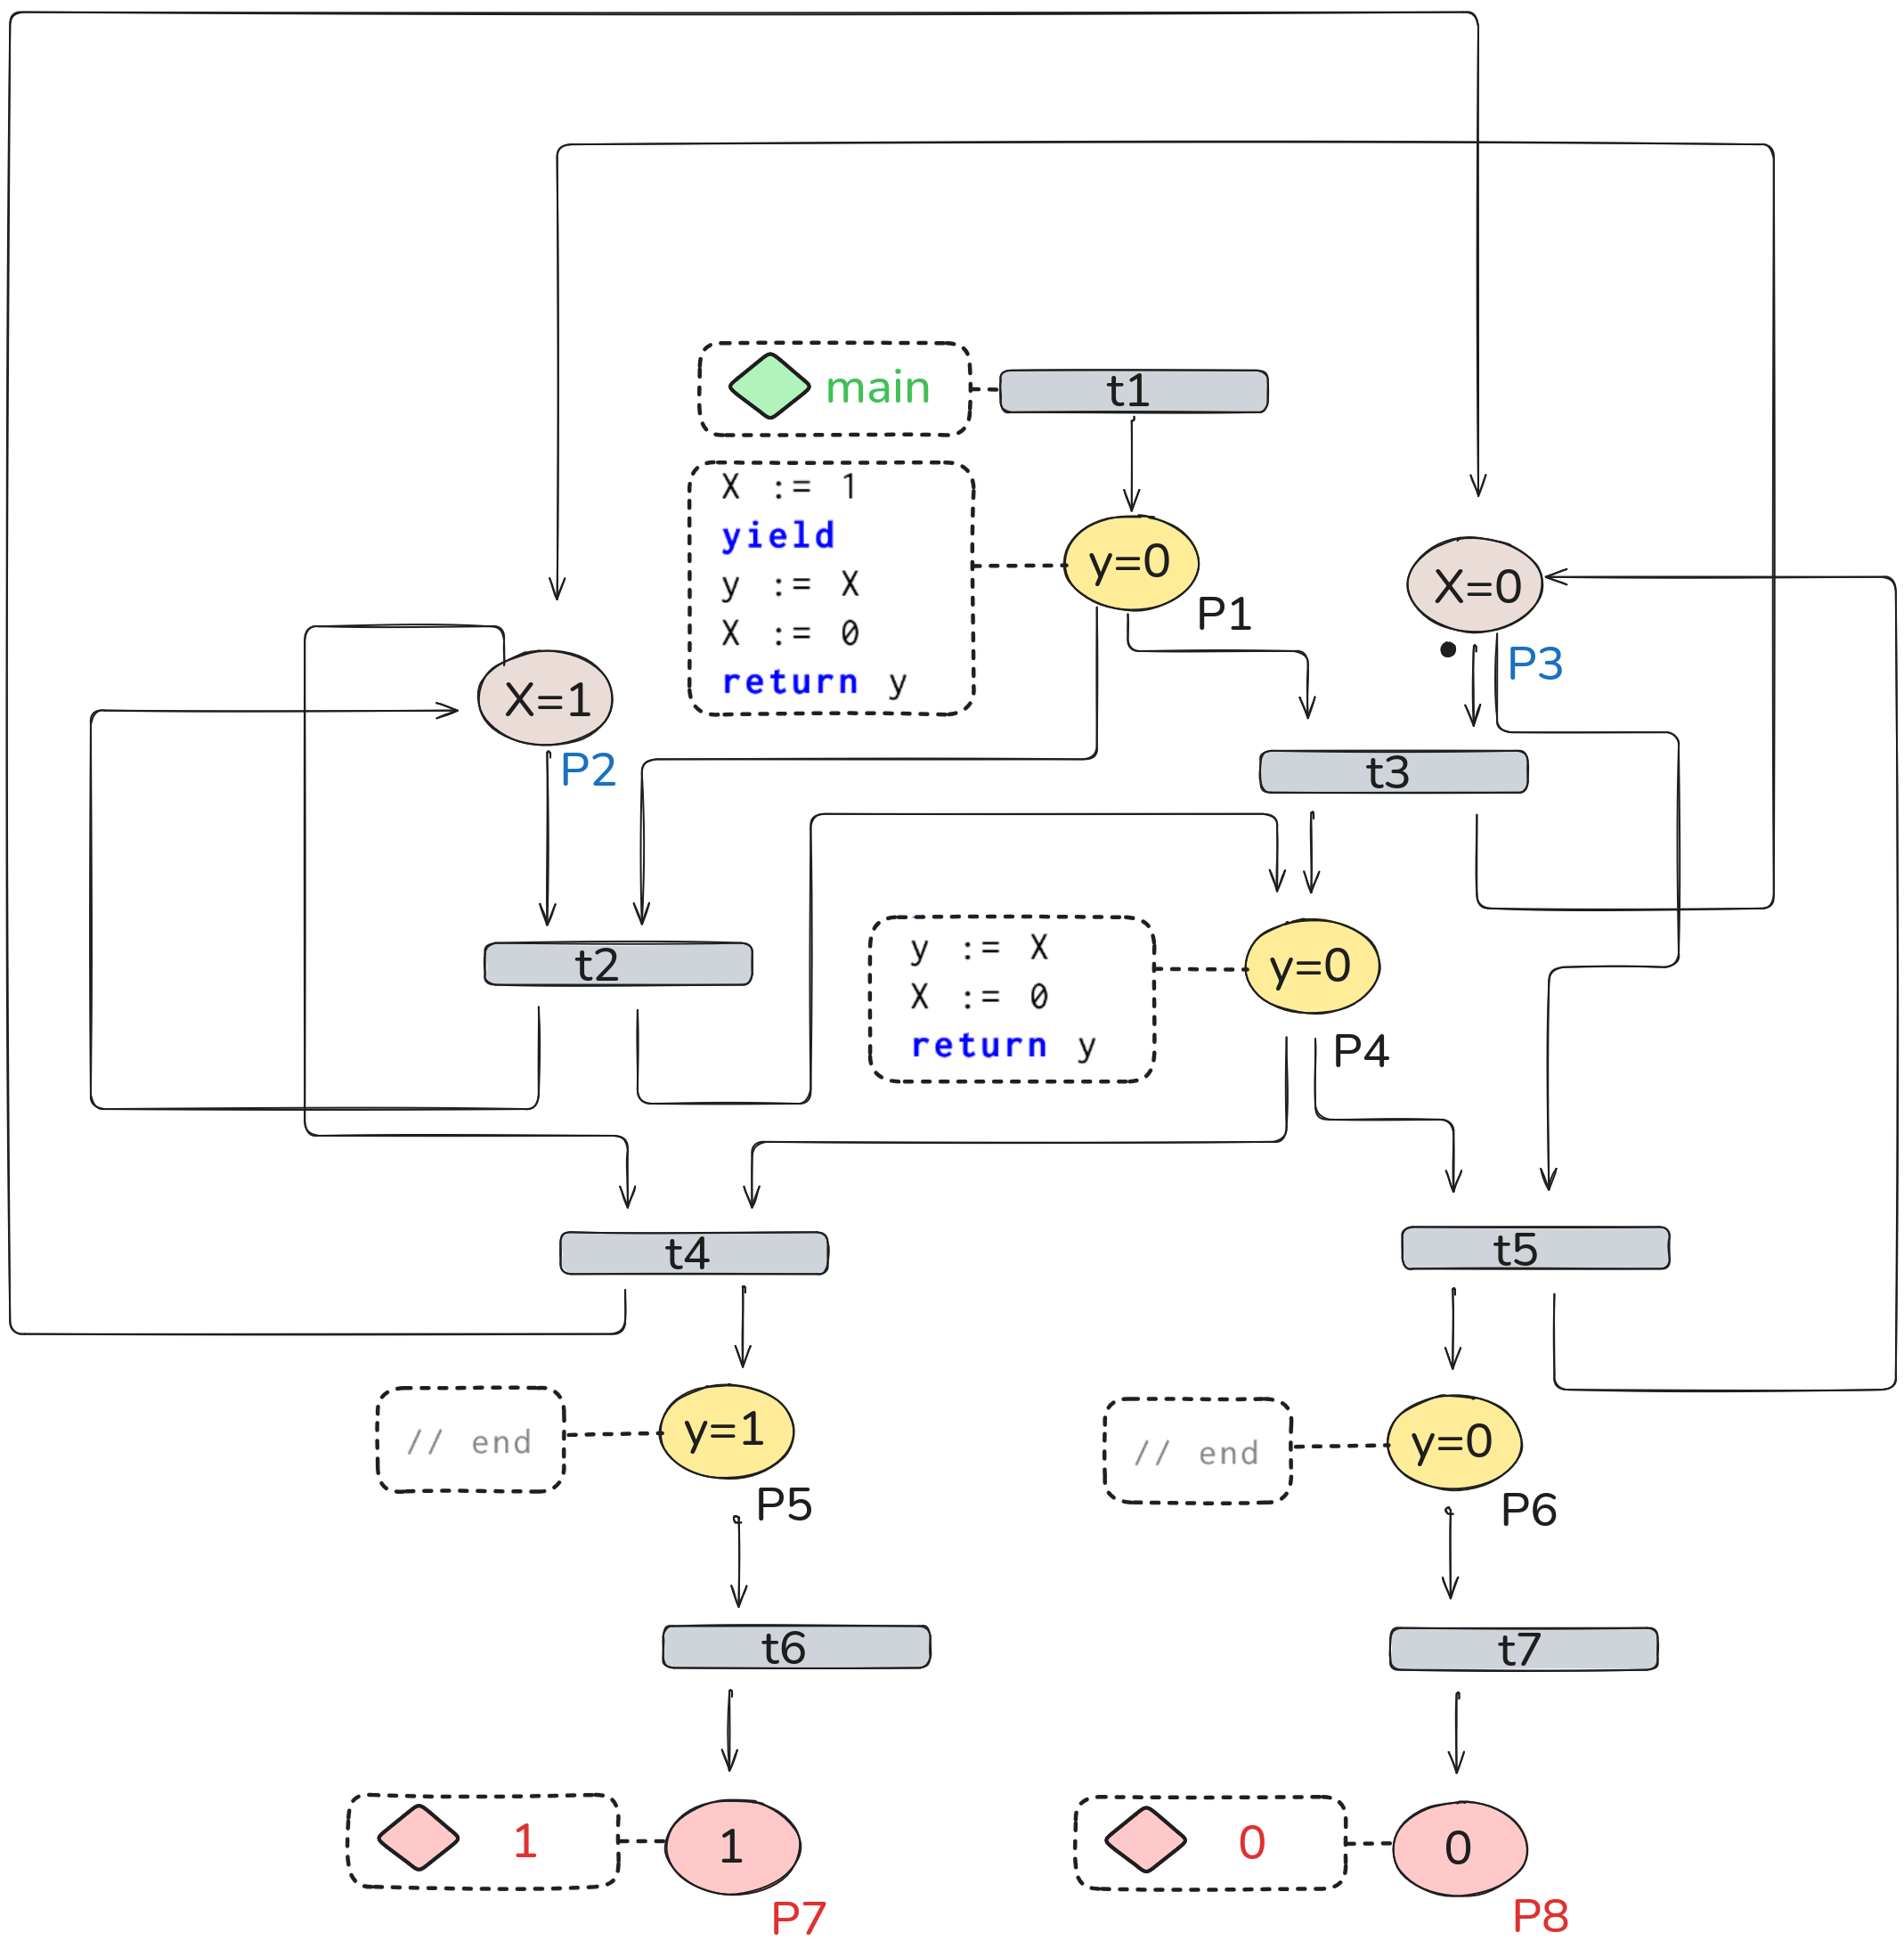
\includegraphics[width=0.7\textwidth]{plots/code_2_PN_with_annotation.png}
	\caption{The PN encoding interleaved executions of the program in Listing~\ref{lst:MotivatingExample2NonSer}.}
	\label{fig:code2ExamplePN}
\end{figure}



	
	
	\item \textbf{Non-serializable set.}  
	Let
	\(\;\mathsf{NonSer}(\mathcal S)=\mathbb N^{|\Sigma|}\setminus \mathsf{Ser}(\mathcal S)\), i.e., all multisets of (${{\color{ForestGreen}\blacklozenge_{\mathit{req}}}/{\color{red}\blacklozenge_{\mathit{resp}}}}$) pairs that \textit{cannot} be obtained via a serial execution of NS $\mathcal S$.
	
	\begin{tcolorbox}[colback=black!5!white, colframe=black, boxrule=1pt]
	\textbf{Example.}
	Regarding the aforementioned program, we automatically generate the following reachability query\footnote{If not for the equality constraints, the problem would have been considered a Petri net \textit{coverability} query, which is easier~\cite{Ra78}.} for the Petri net in Fig.~\ref{fig:code2ExamplePN}, encoding a target semilinear set by imposing the following constraints on the token distribution:
	%
	%Regarding the aforementioned program, we automatically generate the following reachability query~\footnote{If not the equality constraints, the problem would have been considered a \textit{coverability} query which is easier~\cite{Ra78}.} for the Petri net in Figure~\ref{fig:code2ExamplePN} we encode a target semilinear set with the following constraints on the token distribution:
	%
	\[
	\mathcal {F}: \quad P_1 = 0 \wedge 
	\textcolor{blue}{P_2} \ge 0 \wedge \textcolor{blue}{P_3} \ge 0  \wedge P_4 = 0
	\wedge P_5 = 0 \wedge P_6 = 0 \wedge \textcolor{red}{P_7} \ge 0 \wedge \textcolor{red}{P_8} \ge 1.
	\]
	
	This set requires no tokens on $P_1,P_4,P_5,P_6$, at least one token on $\textcolor{red}{P_8}$ (i.e., a response {\color{red}$\blacklozenge_0$}), and any number of tokens on $\textcolor{blue}{P_2},\textcolor{blue}{P_3},\textcolor{red}{P_7}$. 
	%
%	Note that \(\textcolor{red}{P_8} \ge 1\) requires at least one {\color{red}$\blacklozenge_0$}, as expected (see \Cref{sec:introduction}).
	\end{tcolorbox} 
	
	
%	\item \textbf{Reachability encoding.}  
	
	
	\item \textbf{Decision \& validation.}
	We ask whether there exists a marking \(M\) of \(N_{\mathrm{int}}(\mathcal S)\) such that \(M \models \mathcal {F}\), i.e.,
	\[
	M_0 \xrightarrow{}^{*} M
	\quad\wedge\quad
	\pi(M)\in \mathsf{NonSer}(\mathcal S).
	\]
	
	\begin{itemize}
		\item [\sat]: yields a counterexample interleaving \(M\) with
		\(\pi(M)\notin \mathsf{Ser}(\mathcal S)\), validated by simulation of the NS.
%		We validate a reachable trace and embed it into the NS semantics, yielding a valid interleaving that produces request/response pairs unattainable under any serial execution.
		
		\item [\unsat]: yields an inductive invariant of
		\(N_{\mathrm{int}}\), back-translated to an NS-level proof of serializability 
%		(Appendix~\ref{appendix:ns-serializable}).
%		
%		which back-translates to an NS-level proof of
%		serializability 
%		for \(\mathcal S\)
		%
%		back-translated to a validated by synthesizing an inductive invariant over the interleaving PN, thereby proving that the corresponding semilinear set cannot be realized by any interleaving 
(see an example in Appendix~\ref{appendix:ns-serializable}).
	\end{itemize}

\begin{tcolorbox}[colback=black!5!white, colframe=black, boxrule=1pt]
	\textbf{Example.}
	In our running example, the target semilinear set \(\mathcal {F}\) is, in fact, reachable. For instance, it includes the following marking:
	
	\[
	M^* = \{\textcolor{blue}{P_3}(1),\;\textcolor{red}{P_7}(1),\;\textcolor{red}{P_8}(1)\}
	\]
	
	which is reachable by the PN in Fig.~\ref{fig:code2ExamplePN}. The full firing sequence leading to marking $M^*$ is denoted in Table~\ref{tab:PetriNetFiringCounterexample} (in Appendix~\ref{appendix:non-serializable-execution-example}).
	%
%	As the target set encodes request/response pairs that are \textit{unattainable} via serial executions, and as the PN encodes all possible interleavings, this firing sequence also corresponds as a counterexample demonstrating the program is non-serializable. 
	%
	Specifically, this reachable marking encodes the outputs $\{{\color{ForestGreen}\blacklozenge_\text{main}}/{\color{red}\blacklozenge_0},{\color{ForestGreen}\blacklozenge_\text{main}}/{\color{red}\blacklozenge_1}\}$ which, indeed, can only be induced by a non-serial execution (see~\Cref{sec:introduction}).
\end{tcolorbox} 
%\item \textbf{Validation.}  
%
%	\begin{itemize}
%		
%		\item[\sat]: 
%		See the example in subsec.~\ref{subsec:ns-not-serializable}.
%		
%%		\item[\unsat]: 
%		
%		
%	\item \sat: we validate the reachable trace and project it to the NS semantics to represent a valid interleaving that results into request/response pairs which cannot be attained in serial executions.
%	See example in subsec.~\ref{subsec:ns-not-serializable}.
	
%	\item \unsat:
%	we generate an inductive invariant over the interleaving PN, proving that the semilinear set cannot be attained via an interleaving.
%	See example in subsec.~\ref{subsec:ns-serializable}.
%\end{itemize}

\end{enumerate}

\medskip
\noindent
\textbf{Complexity analysis.}
The core algorithm reduces serializability checking to Petri net reachability with target semilinear sets. 
Since the serial executions form a regular language (step 1), their Parikh image is effectively semilinear by Parikh's theorem, with size exponential in the NFA.
The interleaving Petri net (step 2) has $O(|G| + (|\mathit{REQ}| \times |L|) + (|\mathit{REQ}| \times |\mathit{RESP}|))$ places and $O(|\mathit{REQ}|\times (1+ |\delta| + |\mathit{RESP}|))$ transitions.
The reachability query (step 3) asks whether the Petri net can reach the complement of a semilinear set, which is decidable but \texttt{Ackermann}-complete~\cite{CzWo22}.
Without optimizations, even simple examples can generate Petri nets with hundreds of places and exponentially-sized semilinear constraints, making the approach impractical.
Our optimizations (see subsec.~\ref{sec:optimizations}) \textit{drastically} reduce both the Petri net size and the semilinear set complexity, as we elaborate next.


%\guy{should we add/prove the following?}
%
%\begin{proposition}
%	Let $N_{\mathrm{int}}(\mathcal S)=(P,T,\mathsf{pre},\mathsf{post},M_0)$ be the interleaving Petri net constructed above, and let
%	\[
%	\pi\colon\mathbb N^P\to\mathbb N^{P_R}
%	\]
%	be the projection onto the request/response places $P_R$.  Then
%	\[
%	\mathsf{Int}(\mathcal S)
%	\;=\;
%	\{\;\pi(M)\;\mid\;M_0\xrightarrow{*}M\}.
%	\]
%\end{proposition}


\subsection{Optimizations}
\label{sec:optimizations}

%\todo{check}

We apply four optimizations to the base algorithm to control intermediate blow‐up in the size of both the PN and the constructed semilinear set. 
%
An extensive empirical evaluation of these optimizations appears later on in subsec.~\ref{subsec:optimization-results}.

\medskip
\noindent
\textbf{(1) Bidirectional pruning.}  
When solving Petri net reachability, many places and transitions might be irrelevant to the specific target set.  
	We prune them before symbolic reasoning by combining forward and backward passes:  
	the forward pass over-approximates the places reachable from $M_0$; and symmetrically,   
	the backward pass traverses in reverse from any place that can influence a target constraint (hence over-approximating the places that can contribute to it).
	We iteratively remove non-forward-reachable and
	non-backward-relevant places and transitions, to a fixed point.  
	Appendix~\ref{appendix:BidirectionalProof} illustrates this (Fig.~\ref{fig:bidirectional_pruning}) and proves soundness (Theorem~\ref{thm:bidirectional-pruning}):


%\guy{check with mark (M0 projected on P or P'?)}

\begin{theorem}[Bidirectional Pruning Soundness]
	\label{thm:bidirectional-pruning}
	Let $N = (P, T, Pre, Post, M_0)$ be a Petri net and $S$ a target set.  
	Let $N' = (P',T',\,\Pre|_{P'\times T'},\,\Post|_{P'\times T'},\,M_0|_{P'})$ be the pruned net.  
	Then $S$ is reachable from $N$ iff it is reachable from $N'$.
\end{theorem}
%
%We depict this in Fig.~\ref{fig:bidirectional_pruning}, and prove Theorem~\ref{thm:bidirectional-pruning} in Appendix~\ref{appendix:BidirectionalProof}.
% (see the proof in Appendix~\ref{appendix:BidirectionalProof}).
%

% \medskip
% \noindent\textit{\textbf{Intuition.}}
% Before any heavy symbolic reasoning takes place, we apply bidirectional pruning on the underlying PN.  In the forward pass, we traverse from the initial marking to identify an over-approximation of all places and transitions that could ever fire; in the backward pass, we traverse backward from any place that can influence a target constraint, and identify over-approximations on transitions and places that cannot contribute to reaching it.  By iteratively repeating forward passes and backward passes until convergence, we remove every component of the net that cannot both originate and contribute to the reachable target set.  This dramatically shrinks the net in practice, often converting an intractably large model into one small enough for exhaustive analysis.

\medskip
\noindent
\textbf{(2) Semilinear set pruning.}  
A semilinear set $S=\bigcup_{i=1}^m L_i$ with 
	$L_i=\{\,b_i+\sum_{p\in P_i}n_p p \mid n_p\in\mathbb N\}$ may contain redundant 
	period vectors or components.  
	Thus, during construction, we:
	(1) remove any period vector $p\in P_i$ expressible as a nonnegative combination of $P_i\setminus\{p\}$; 
	and (2) drop $L_i$ when $L_i\subseteq L_j$ (for \(i \neq j\)).  
	This pruning keeps formulas compact and solver calls tractable.




% it is common for some inequalities or disjuncts to add no new coverage beyond what other constraints already guarantee.  The redundant‐constraint elimination pass inspects each linear inequality and each disjunct in a disjunctive normal form, testing whether it is implied by the rest.  Any constraint or disjunct found redundant is dropped, ensuring that subsequent intersection, union, and projection operations work on the smallest necessary formula.  This streamlines the logic formula and prevents unnecessary size blow‐ups during solver invocations.

% %
% We replace each period‐basis \(P_i\) by
% \[
% P_i \;:=\;\{\,p\in P_i \mid p\notin\mathsf{Span}(P_i\setminus\{p\})\}
% \],
% Dropping any ``redundant'' periods, and removing any \(L_j\subseteq L_i\) for \(i\neq j\), iterating to a fixed point so no two components subsume one another.

\medskip
\noindent
\textbf{(3) Generating fewer constraints.}  
When computing the Parikh image of a regular expression as a semilinear set,
	most regex operations can be implemented without an exponential blow-up.
	However, the Kleene star is a notable exception. Given $S=\bigcup_{i=1}^m L_i$,  the Kleene closure $S^\ast$ can be expressed as a semilinear set by: 
	\[
	S^\ast=\bigcup_{I \subseteq \{1,...,m\}} 
	\Big\{\sum_{i \in I} b_i + \sum_{p \in \bigcup_{i \in I} (P_i\cup \{b_i\})} n_p p\Big\},
	\]
	yielding $2^m$ components. To mitigate this:
	(i) if $L_i=\{b_i\}$ (period-less component), factor it out, star the rest, then add $b_i$ as a period;  
	(ii) if $L_i=\{\sum_{p\in P_i}n_pp\}$ (zero base), likewise star the rest and add each $p\in P_i$ as a period vector to the resulting set.  
	Each such case halves the component count and circumvents exponential blow-ups.




% Let $\mathrm{comp}(S)=\{L_1,\dots,L_m\}$ 
% be the multiset of linear components of the semilinear set 
% \(\displaystyle S=\bigcup_{i=1}^m L_i\), where each 
% \(\;L_i=b_i+\langle P_i\rangle\) with \(b_i\in\mathbb N^d\) and 
% \(P_i\subseteq\mathbb N^d\).  Define the pruning operator
% \[
% \mathrm{new}(\mathcal C)
% \;=\;
% \bigcup\bigl\{\,L\in\mathcal C \;\bigm|\;\nexists\,L'\in\mathcal C\setminus\{L\}:\;L'\subsetneq L\bigr\},
% \]
% which removes any component strictly containing another.  
% %
% \guy{Nicolas is it clear we mean that we fix their semilinear "meaning" of the regex operations? For example, + is union etc..}
% Then, we replace the naive semilinear‐set operations by
% \[
% S\;+\;T
% \;=\;
% \mathrm{new}\bigl(\mathrm{comp}(S)\,\cup\,\mathrm{comp}(T)\bigr),
% \]
% \[
% S\;\cdot\;T
% \;=\;
% \mathrm{new}\Bigl(\{\,L_i\cdot L'_j \mid L_i\in\mathrm{comp}(S),\;L'_j\in\mathrm{comp}(T)\}\Bigr),
% \]
% where for
% \(\;L_i=b_i+\langle P_i\rangle,\;L'_j=b'_j+\langle P'_j\rangle\) we set
% $
% L_i\cdot L'_j
% =\;(b_i+b'_j)\;+\;\langle\,P_i\cup P'_j\,\rangle.
% $
% Finally, for Kleene‐star and plus on the regex side one similarly applies
% \(\mathrm{new}(\cdot)\) to the collection of ``folded” components instead of
% building all intermediate ones:
% \[
% S^*
% =\mathrm{new}\Bigl(\bigcup_{k\ge0}\bigl(\mathrm{comp}(S)\bigr)^k\Bigr),
% \qquad
% S^+
% =S\cdot S^*.
% \]

% \medskip
% \noindent\textit{\textbf{Intuition.}}
% %
% During set construction --- especially when introducing new existentially‐quantified variables or combining transition effects, we selectively avoid generating any marking that would strictly dominate an already‐seen solution.  In effect, whenever a candidate disjunct would yield a superset of an existing one, it is skipped entirely.  This ``generate‐less” heuristic stops the proliferation of large, overlapping regions in the semilinear description.  In benchmarks with large state spaces, it can reduce the number of intermediate branches by orders of magnitude.

\medskip
\noindent
\textbf{(4) Strategic Kleene elimination order.} 
%
We use \textit{Kleene's algorithm}~\cite{Kl56} to translate the serializability NFA into a regex.
% 
The size of the generated semilinear set is not only impacted by how the
	semilinear set operations are implemented, but also by what \textit{specific} regular
	expression is given as input: a single regular language may be represented by a
	number of equivalent regexes, each of different complexity.
	%
	In particular, as Kleene star can cause a large blow-up in the semilinear set size,
	we are especially sensitive to the \emph{star height} of the generated regex.
	%
	Naive Kleene elimination may introduce many nested stars.  
	We reduce this by strategically choosing to eliminate lower-degree states first:
	\[
	q^*=\arg\min_{q\in Q}\bigl(|\delta^A_{\mathrm{in}}(q)|+|\delta^A_{\mathrm{out}}(q)|\bigr),
	\]
	 
	
	\smallskip
	\noindent
	As we later demonstrate (in~\Cref{sec:evaluation}), our optimizations expedite the search procedure and make the representations significantly more compact. This, in turn, enables deciding serializability for instances that are otherwise intractable.


%\medskip
%\noindent
%\textbf{(4) Strategic Kleene elimination order.}  
%The size of the generated semilinear set is not only impacted by how the
%semilinear set operations are implemented, but also by what specific regular
%expression is given as input: a single regular language may be represented by a
%number of equivalent regexes, each of different complexity.
%%
%In particular, as Kleene star can cause a large blow-up in the semilinear set size,
%we are especially sensitive to the \emph{star height} of the generated regex.
%%
%We use Kleene's algorithm to convert an NFA $\mathcal A=(Q,\Sigma,\delta,q_0,F)$ to a regex, which works by repeated state elimination, choosing one state at a time.
%Naively, when eliminating states in an arbitrary order, Kleene's algorithm may generate regexes with a much greater star height than necessary---a problem
%when converting to semilinear sets.
%%
%Therefore, we heuristically optimize the state elimination order to end up with a smaller regex. Formally, we pick the next state:
%\[
%q^* = 
%\arg\min_{q\in Q'}\bigl(|\delta_{\mathrm{in}}(q)|+|\delta_{\mathrm{out}}(q)|\bigr)
%\]
%where \(Q'\subseteq Q\) are the states remaining to be eliminated, choosing to
%eliminate states with a smaller total degree first.
%%
%This empirically keeps the resulting regexes small.

% \medskip
% \noindent\textit{\textbf{Intuition.}}
% When converting an NFA to a single regex, we pick the next state to eliminate by heuristically choosing the  state with the fewest incoming and outgoing edges.
% This optimization allows for circumventing 
% overblown expressions resulting in naive translations, especially with regard to  Kleene closures (the “\(\mathsf{*}\)” operator).  Instead, we analyze the structure of sub-expressions under the various operators --- estimating their branching factor, and reordering them so that simpler, low‐branching components are expanded first.  
%This adaptive ordering often leads to early detection of fixed points or dead‐ends, preventing the combinatorial explosion that arises when complex loops are expanded prematurely.  
